Nella precedente sezione \ref{subsec:supermercato24StrutturaDatabase} è emersa la necessità di notificare a tutti i dispositivi connessi ogni azione intrapresa da un cliente in tempo reale.
Lo scopo di questo lavoro è valutare la migliore implementazione disponibile e compatibile con lo stack attuale.
Questo progetto è stato rinominato ``SmIoT'' dall'unione di ``Supermercato'' e ``IoT''.

\subsection{Analisi iniziale}
\label{subsec:smiotAnalisi}

\noindent
I requisiti iniziali sono:
\begin{itemize}
  \item sincronizzazione inserimento/modifica/eliminazione di un prodotto nel carrello
  \item notificare inserimento/eliminazione di un prodotto preferito
  \item notificare la transazione dello stato dell'ordine
  \item sincronizzare gli slot orari di ogni supermercato
\end{itemize}

\bigskip
\noindent
I possibili sviluppi dall'implementazione potrebbero essere:
\begin{itemize}
  \item creazione di una chat per l'assistenza clienti
  \item utilizzare notifiche push a fini di marketing
  \item fornire informazioni dettagliate sull'arrivo del fattorino
  \item analizzare i clienti connessi in tempo reale
\end{itemize}

Tutti i valori sono associati per utente e devono essere isolati ai suoi dispositivi.
L'utilizzo del servizio da parte dei dispositivi mobile, condiviso tra app e sito responsive, si attesta sul 50\%, mentre gli ordini fatti solo da app sono circa il 30\%.
Con questi dati si è scelto di non sottovalutare le difficoltà della \verb+UX+ dei \textit{client} non desktop.

\subsection{Implementazione}
\label{subsec:smiotImplementazione}

Attualmente tutti i requisiti sono gestiti tramite chiamate \verb+RESTful+ descritte nella sezione \ref{subsec:supermercato24StrutturaArchitettura}.
Il cambio di paradigma, verso una tipologia asincrona, dovrebbe migliorare l'esperienza generale del cliente aumentando la soddisfazione.

Grazie all'esperienza maturata con il precedente progetto della sezione \ref{sec:socksberry}, inizialmente era stato considerato l'utilizzo del \verb+WebSocket+.
Il primo mockup, infatti, utilizzava un'implementazione simile, ma i risultati, soprattutto verso i dispositivi smart, non erano abbastanza soddisfacenti.
La possibile degradazione della banda e il sovraccarico delle connessioni non garantivano la scalabilità e la qualità prevista inizialmente.

Si è dovuto cercare un protocollo alternativo che potesse garantire la stabilità necessaria per questi dispositivi.
Sono stati analizzati diversi protocolli quali: \verb+AMQP+, \verb+STOMP+ e \verb+MQTT+.
Il protocollo \verb+MQTT+, descritto nella sezione \ref{sec:mqtt}, teoricamente poteva soddisfare i requisiti iniziali.

È stato sviluppato un applicativo \verb+NodeJs+  (\textit{``broker''}) sul \textit{server} di produzione connesso con il KeyValue tramite una comunicazione \textit{publish}/\textit{subscribe} per ricevere gli aggiornamenti di ogni utente.
Il programma è riportato in appendice \ref{app:smiot_controller}.

Ogni \textit{client} una volta connesso e autenticato al sito, effettua l'\textit{handshake} verso il \textit{broker} tramite il \textit{token} di sessione che lo identifica all'interno del sistema.
Tramite protocollo \verb+MQTT+ viene concordato il giusto livello di \verb+QoS+ in base alla sua connessione.
Alla notifica di un evento, viene effettuato il \textit{dispatch} da parte del \textit{broker} all'utente appropriato, seguendo questo flow:
\begin{enumerate}
  \item connessione del dispositivo \textbf{A} del cliente Foo
  \item connessione del dispositivo \textbf{B} del cliente Foo
  \item connessione del dispositivo \textbf{C} del cliente Foo
  \item il dispositivo \textbf{A} aggiunge/modifica/elimina un prodotto/risorsa chiamata PUT/DELETE
  \item il controller Php effettua l'operazione del prodotto/risorsa e ``pubblica'' il relativo evento
  \item disconnessione del dispositivo \textbf{C} del cliente Foo
  \item il KeyValue consegna il messaggio al broker
  \item il broker spedisce il messaggio al dispositivo \textbf{B}
  \item il dispositivo \textbf{B} conferma il messaggio ed aggiorna le proprie risorse
\end{enumerate}

\begin{figure}[H]
  \centering
  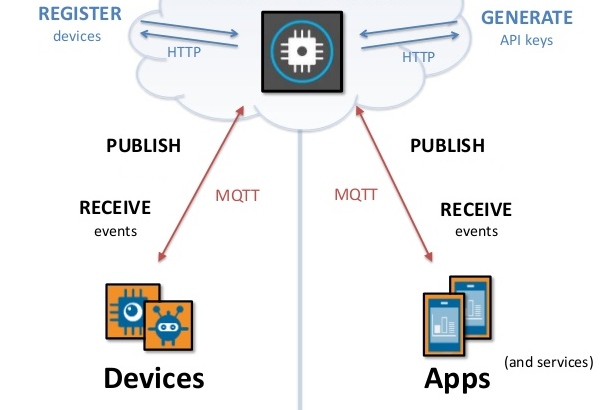
\includegraphics[width=0.95\linewidth, keepaspectratio]{smiot_uml}
  \caption{Modello delle connessioni del progetto SmIoT}
  \label{fig:smiotUml}
\end{figure}

La possibilità di riutilizzare la stessa connessione \verb+MQTT+ per incapsulare le chiamate \verb+RESTful+ è ancora in fase embrionale.
Con questa possibilità si potrebbe sfruttare la comunicazione già instaurata invece di crearne una nuova per intraprendere l'azione.

\subsection{Difficoltà affrontate}
\label{subsec:smiotDifficolta}

Data la complessità dell'operazione, la migrazione è attualmente in fase di test; controllando la compatibilità con tutti i dispositivi.
Per evitare problemi di regressione, il modello dati non è stato variato completamente, permettendo di ripristinare le vecchie funzionalità dinamicamente.

Non è ancora possibile cambiare il \verb+QoS+ una volta connesso: il passaggio dal \verb+Wi-Fi+ al \verb+3G+ non fa aumentare il livello di qualità del servizio.
Si è scelto di effettuare nuovamente la connessione negoziando la qualità del servizio corretta.

Grazie ai ping \textit{KeepAlive} inviati dai vari dispositivi si possono interrompere le connessioni in esubero o fallite.

Attualmente l'1\% degli ordini mensili viene confermato in contemporanea tra due o più dispositivi e solo il primo viene confermato.
Si è scelto di applicare un \textit{mutex} alla risorsa condivisa ``carrello'' e lanciare un errore al tentativo di creazione contemporanea.
La sincronizzazione di questi così poco influenti non è stata ritenuta necessaria.

\subsection{Conclusioni}
\label{subsec:smiotConclusioni}

Dall'analisi dei dati, risulta che circa il 10\% degli ordini viene effettuato con una combinazione di più dispositivi.
Alcuni esempi potrebbero essere:
\begin{itemize}
  \item creazione della spesa durante il lavoro e relativa conferma dell'ordine a casa
  \item apertura dell'e-mail ``conferma account'' dal browser a seguito di una registrazione tramite app
  \item apertura delle e-mail \verb+CRM+ (\textit{Customer relationship management}) dal browser
\end{itemize}

Sincronizzando i dati tra questi \textit{device} non è più necessario, da parte dell'utente, ricaricare il proprio applicativo per notare le modifiche, diminuendo anche le chiamate verso il \textit{server}.
Inoltre l'introduzione graduale di queste feature, grazie al protocollo appropriato, non comporta nessun degrado della qualità dell'esperienza utente.
